\documentclass[../ImageClassifier.tex]{subfiles}

\begin{document}
    To get an overview of the classifier accuracy a network with the keywords cat and dog was trained, because there is a testing set with this keywords on \href{https://www.kaggle.com/tongpython/cat-and-dog?}{www.kaggle.com}.
    The results with search engines trained network is shown in table \ref{table:results cat and dog} below.
    \newline
    \begin{table}[ht!]
        \begin{center}
            \begin{tabular}{{l | c }}
                \centering
                total images & 2025\\
                threshold images & 1843\\
                threshold missed images & 182\\
                correctly classified images & 1838\\
                misclassified images & 5\\
                \hline
                total accuracy & 90.77\% \\
                threshold accuracy & 99.73\% \\
            \end{tabular}
        \end{center}
        \caption{Results of cat and dog testing set}
        \label{table:results cat and dog}
    \end{table}\\
    From 2025 pictures remain 1843 predicted images with a threshold over 99\%, all of the other images counts as misclassified and shown in the total accuracy of 90.77\%.
    But the accuracy of threshold images is at 99.73\%.
    This result shows the importance of a high threshold.
    \newline
    Furthermore, for detecting the localization the toolchain applies automatically \ac{grad-cam} as shown in figures \ref{fig:grad cam cat and dog} and \ref{fig:grad cam pen}.
    \begin{figure}[H]
        \begin{subfigure}{.32\textwidth}
          \centering
          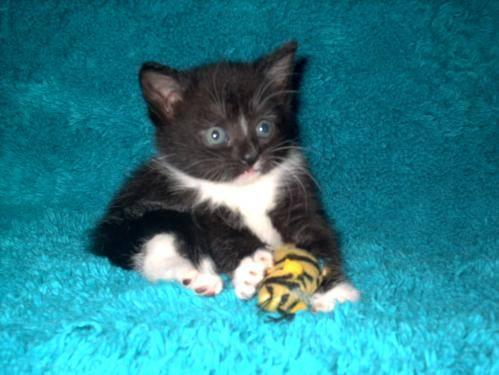
\includegraphics[height=2.5cm, width=2.5cm]{./attachments/results/19-cat.jpg}
          \caption{original image}
          \label{fig:original image}
        \end{subfigure}
        \begin{subfigure}{.32\textwidth}
          \centering
          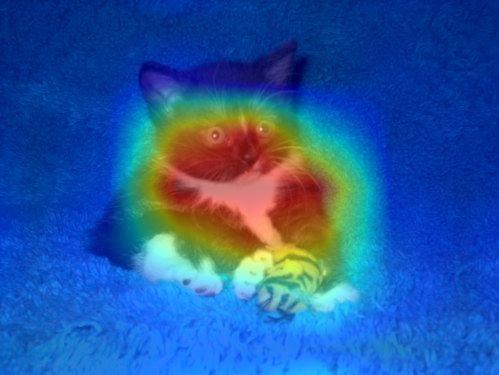
\includegraphics[height=2.5cm, width=2.5cm]{./attachments/results/19-cat-grad.jpg}
          \caption{superimposed image}
          \label{fig:heatmap activasion}
        \end{subfigure}
        \begin{subfigure}{.32\textwidth}
            \centering
            
\includegraphics[height=2.5cm, width=2.5cm]{./attachments/results/19-cat-seg.jpg}
            \caption{segmentation}
            \label{fig:heatmap resized}
        \end{subfigure}
        \caption{Results of \ac{grad-cam} on one image from \href{https://www.kaggle.com/tongpython/cat-and-dog?}{dog and cat testing set}}
        \label{fig:grad cam cat and dog}
    \end{figure}
    \begin{figure}[H]
        \begin{subfigure}{.32\textwidth}
          \centering
          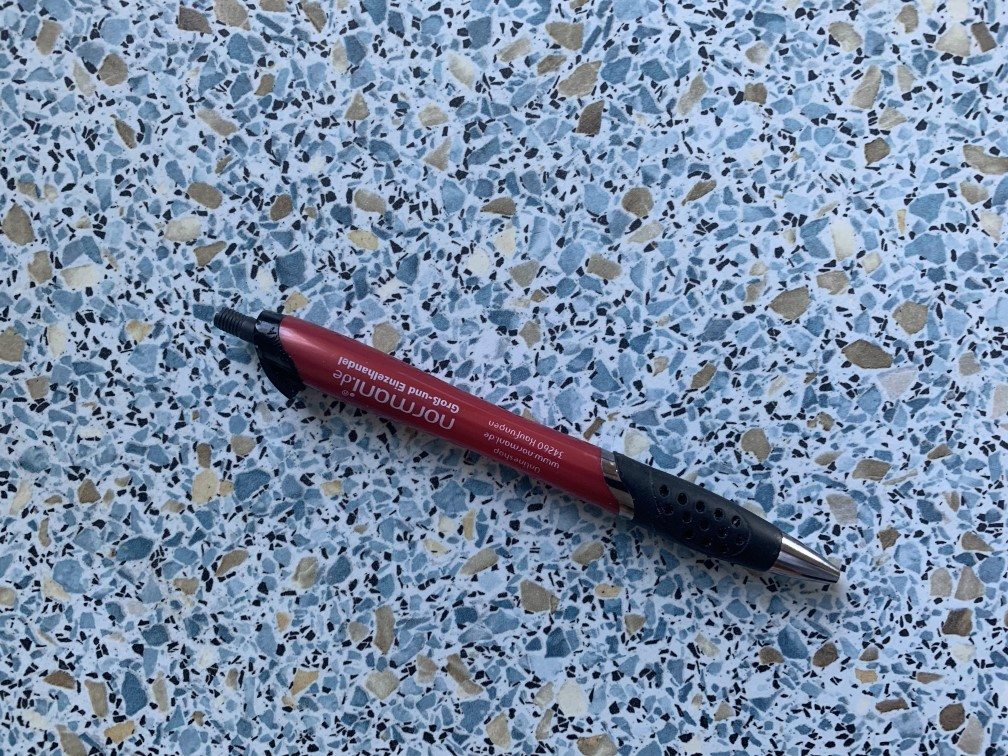
\includegraphics[height=2.5cm, width=2.5cm]{./attachments/results/5-pen.jpg}
          \caption{original image}
          \label{fig:original image}
        \end{subfigure}
        \begin{subfigure}{.32\textwidth}
          \centering
          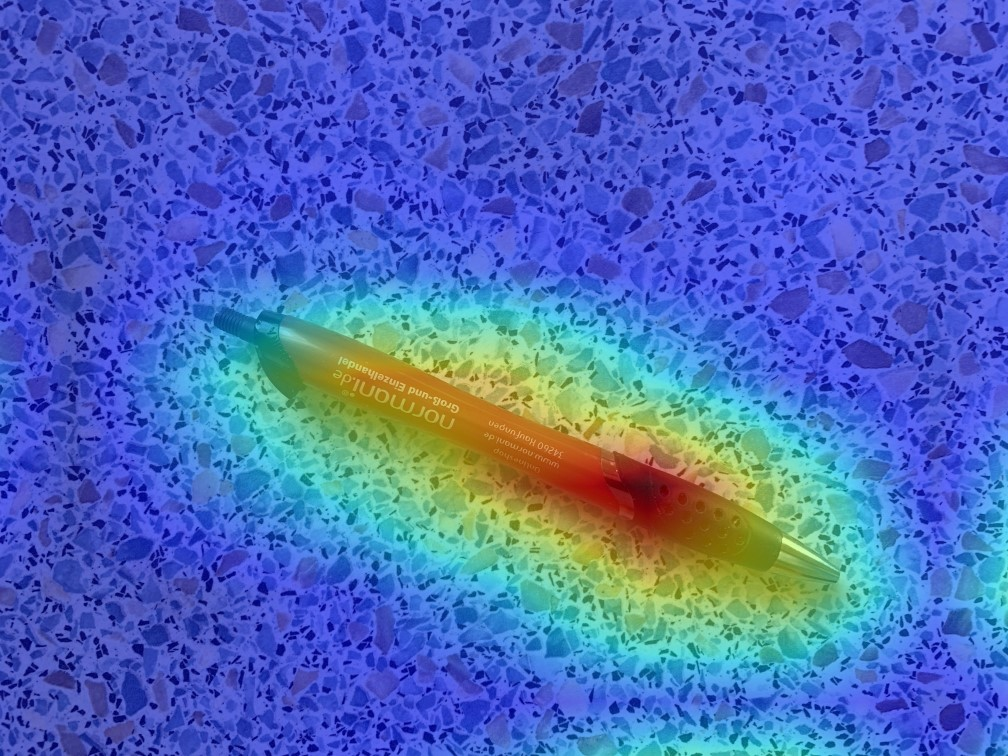
\includegraphics[height=2.5cm, width=2.5cm]{./attachments/results/5-pen-grad.jpg}
          \caption{superimposed image}
          \label{fig:heatmap activasion}
        \end{subfigure}
        \begin{subfigure}{.32\textwidth}
            \centering
            
\includegraphics[height=2.5cm, width=2.5cm]{./attachments/results/5-pen-seg.jpg}
            \caption{segmentation}
            \label{fig:heatmap resized}
        \end{subfigure}
        \caption{Results of \ac{grad-cam} with a pen}
        \label{fig:grad cam pen}
    \end{figure}
    \clearpage
    For every predicted image, the original, the superimposed and the segmentation image are stored in the results directory.
    As shown in figure \ref{fig:grad cam cat and dog} the localization is quite well interpreted, but the results of the localization are very dependent on the background as shown in figure \ref{fig:grad cam rug}.
    \begin{figure}[ht!]
        \begin{subfigure}{.32\textwidth}
          \centering
          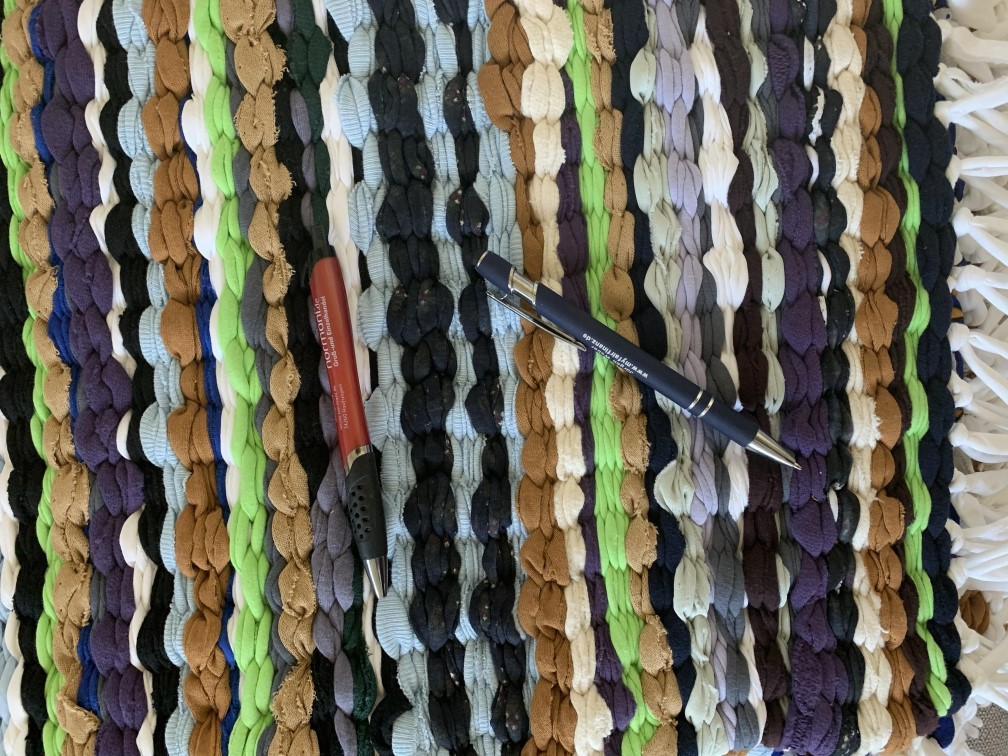
\includegraphics[height=2.5cm, width=2.5cm]{./attachments/results/6-pen.jpg}
          \caption{original image}
          \label{fig:original image}
        \end{subfigure}
        \begin{subfigure}{.32\textwidth}
          \centering
          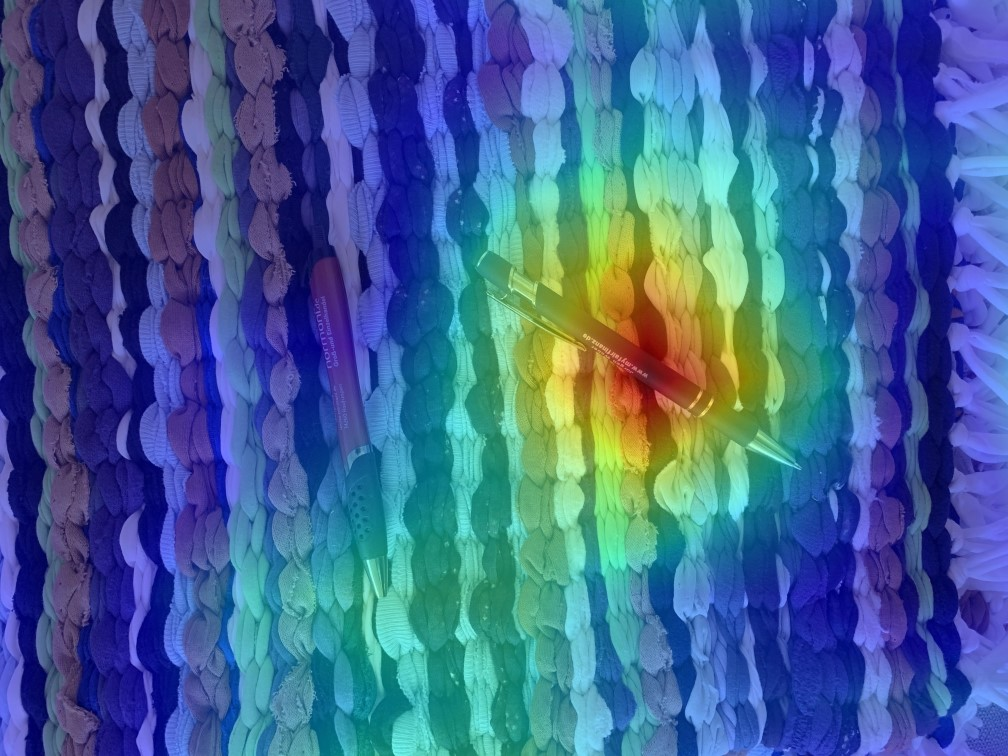
\includegraphics[height=2.5cm, width=2.5cm]{./attachments/results/6-pen-grad.jpg}
          \caption{superimposed image}
          \label{fig:heatmap activasion}
        \end{subfigure}
        \begin{subfigure}{.32\textwidth}
            \centering
            
\includegraphics[height=2.5cm, width=2.5cm]{./attachments/results/6-pen-seg.jpg}
            \caption{segmentation}
            \label{fig:heatmap resized}
        \end{subfigure}
        \caption{Results of \ac{grad-cam} on an image with two pens with a rug in background}
        \label{fig:grad cam rug}
    \end{figure}
    \newline 
    Also it`s very difficult to locate transparent things like a triangle ruler with a background pattern as shown in figure \ref{fig:grad cam triangle}.
    \begin{figure}[ht!]
        \begin{subfigure}{.32\textwidth}
          \centering
          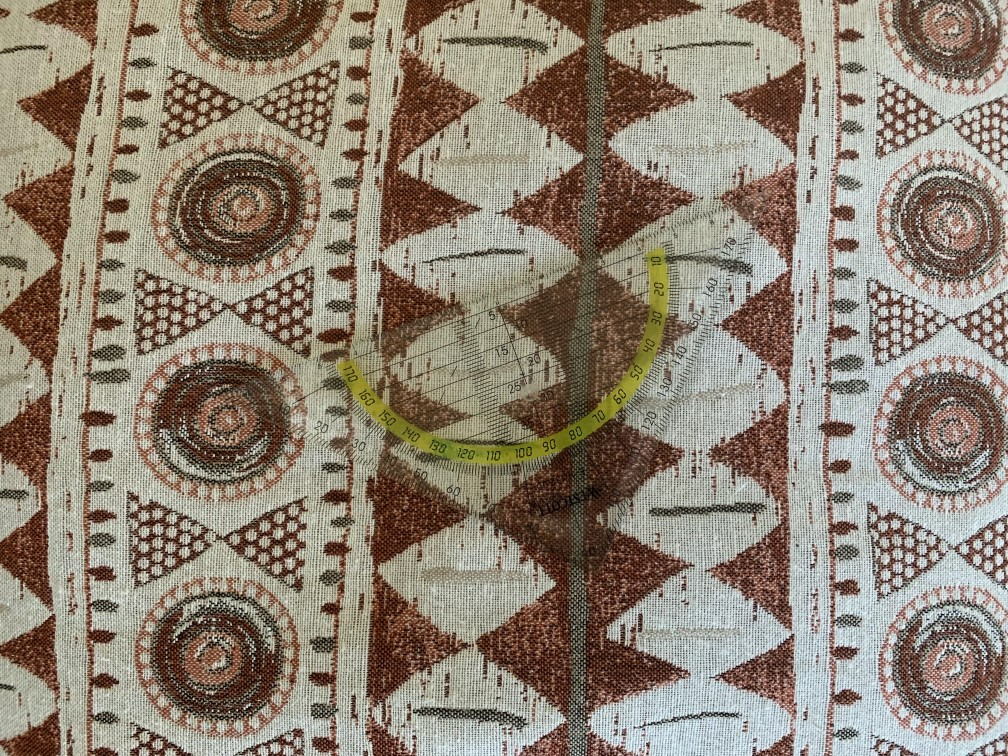
\includegraphics[height=2.5cm, width=2.5cm]{./attachments/results/12-triangle ruler.jpg}
          \caption{original image}
          \label{fig:original image}
        \end{subfigure}
        \begin{subfigure}{.32\textwidth}
          \centering
          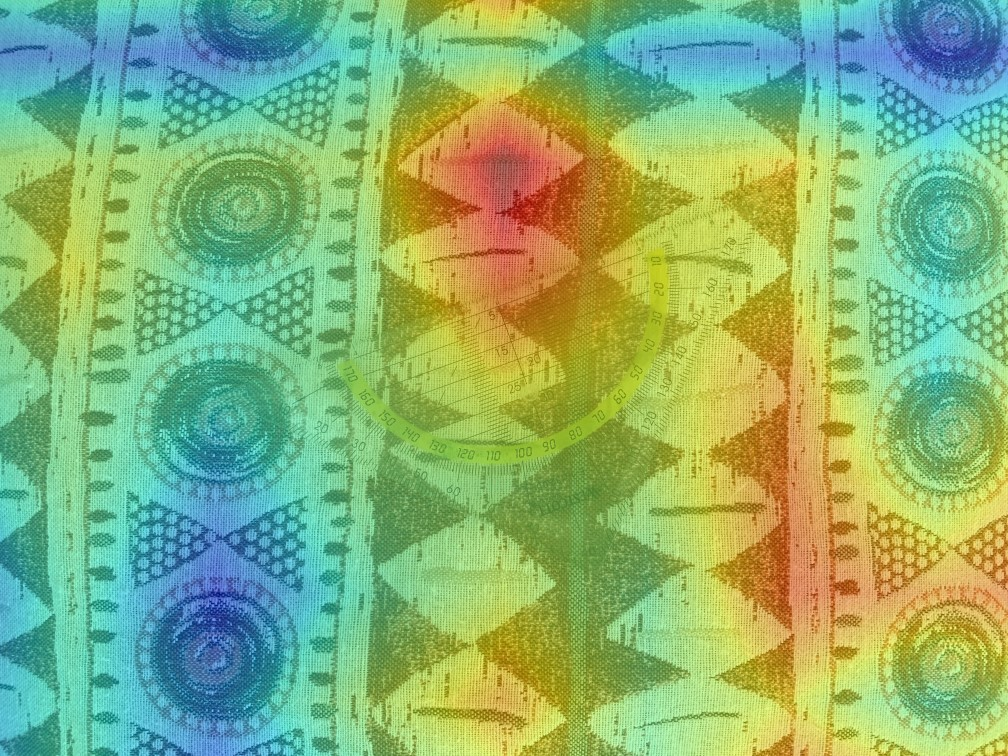
\includegraphics[height=2.5cm, width=2.5cm]{./attachments/results/12-triangle ruler-grad.jpg}
          \caption{superimposed image}
          \label{fig:heatmap activasion}
        \end{subfigure}
        \begin{subfigure}{.32\textwidth}
            \centering
            
\includegraphics[height=2.5cm, width=2.5cm]{./attachments/results/12-triangle ruler-seg.jpg}
            \caption{segmentation}
            \label{fig:heatmap resized}
        \end{subfigure}
        \caption{Results of \ac{grad-cam} on an image with two pens with a rug in background}
        \label{fig:grad cam triangle}
    \end{figure}
    \newline
    Finally a prediction was made with several learned classes to test what happens with the prediction and localization.
    The toolchain automatically select the class with the highest prediction accuracy like in figure \ref{fig:grad cam mixed} the calculator.
    \begin{figure}[H]
      \begin{subfigure}{.32\textwidth}
        \centering
        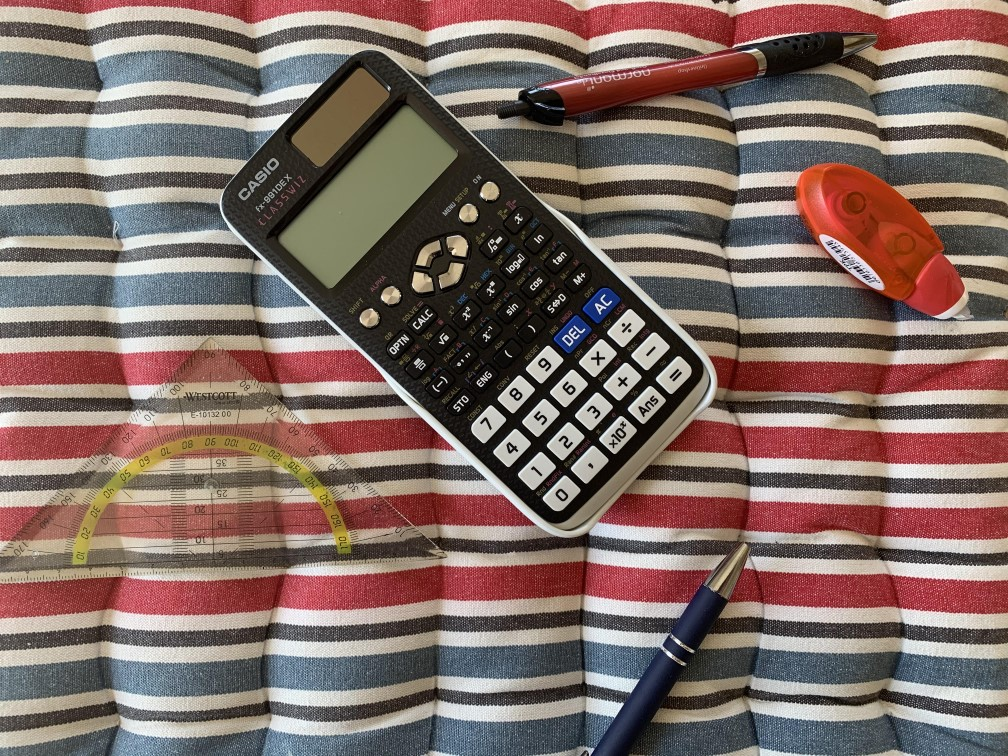
\includegraphics[height=2.5cm, width=2.5cm]{./attachments/results/0-calculator.jpg}
        \caption{original image}
        \label{fig:original image}
      \end{subfigure}
      \begin{subfigure}{.32\textwidth}
        \centering
        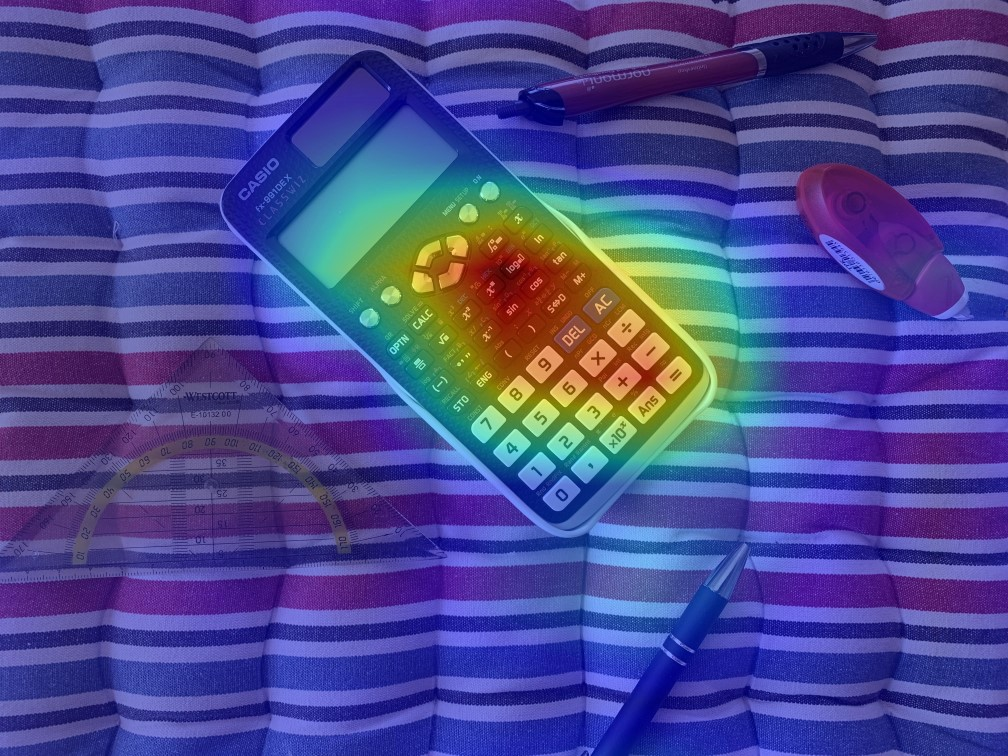
\includegraphics[height=2.5cm, width=2.5cm]{./attachments/results/0-calculator-grad.jpg}
        \caption{superimposed image}
        \label{fig:heatmap activasion}
      \end{subfigure}
      \begin{subfigure}{.32\textwidth}
          \centering
          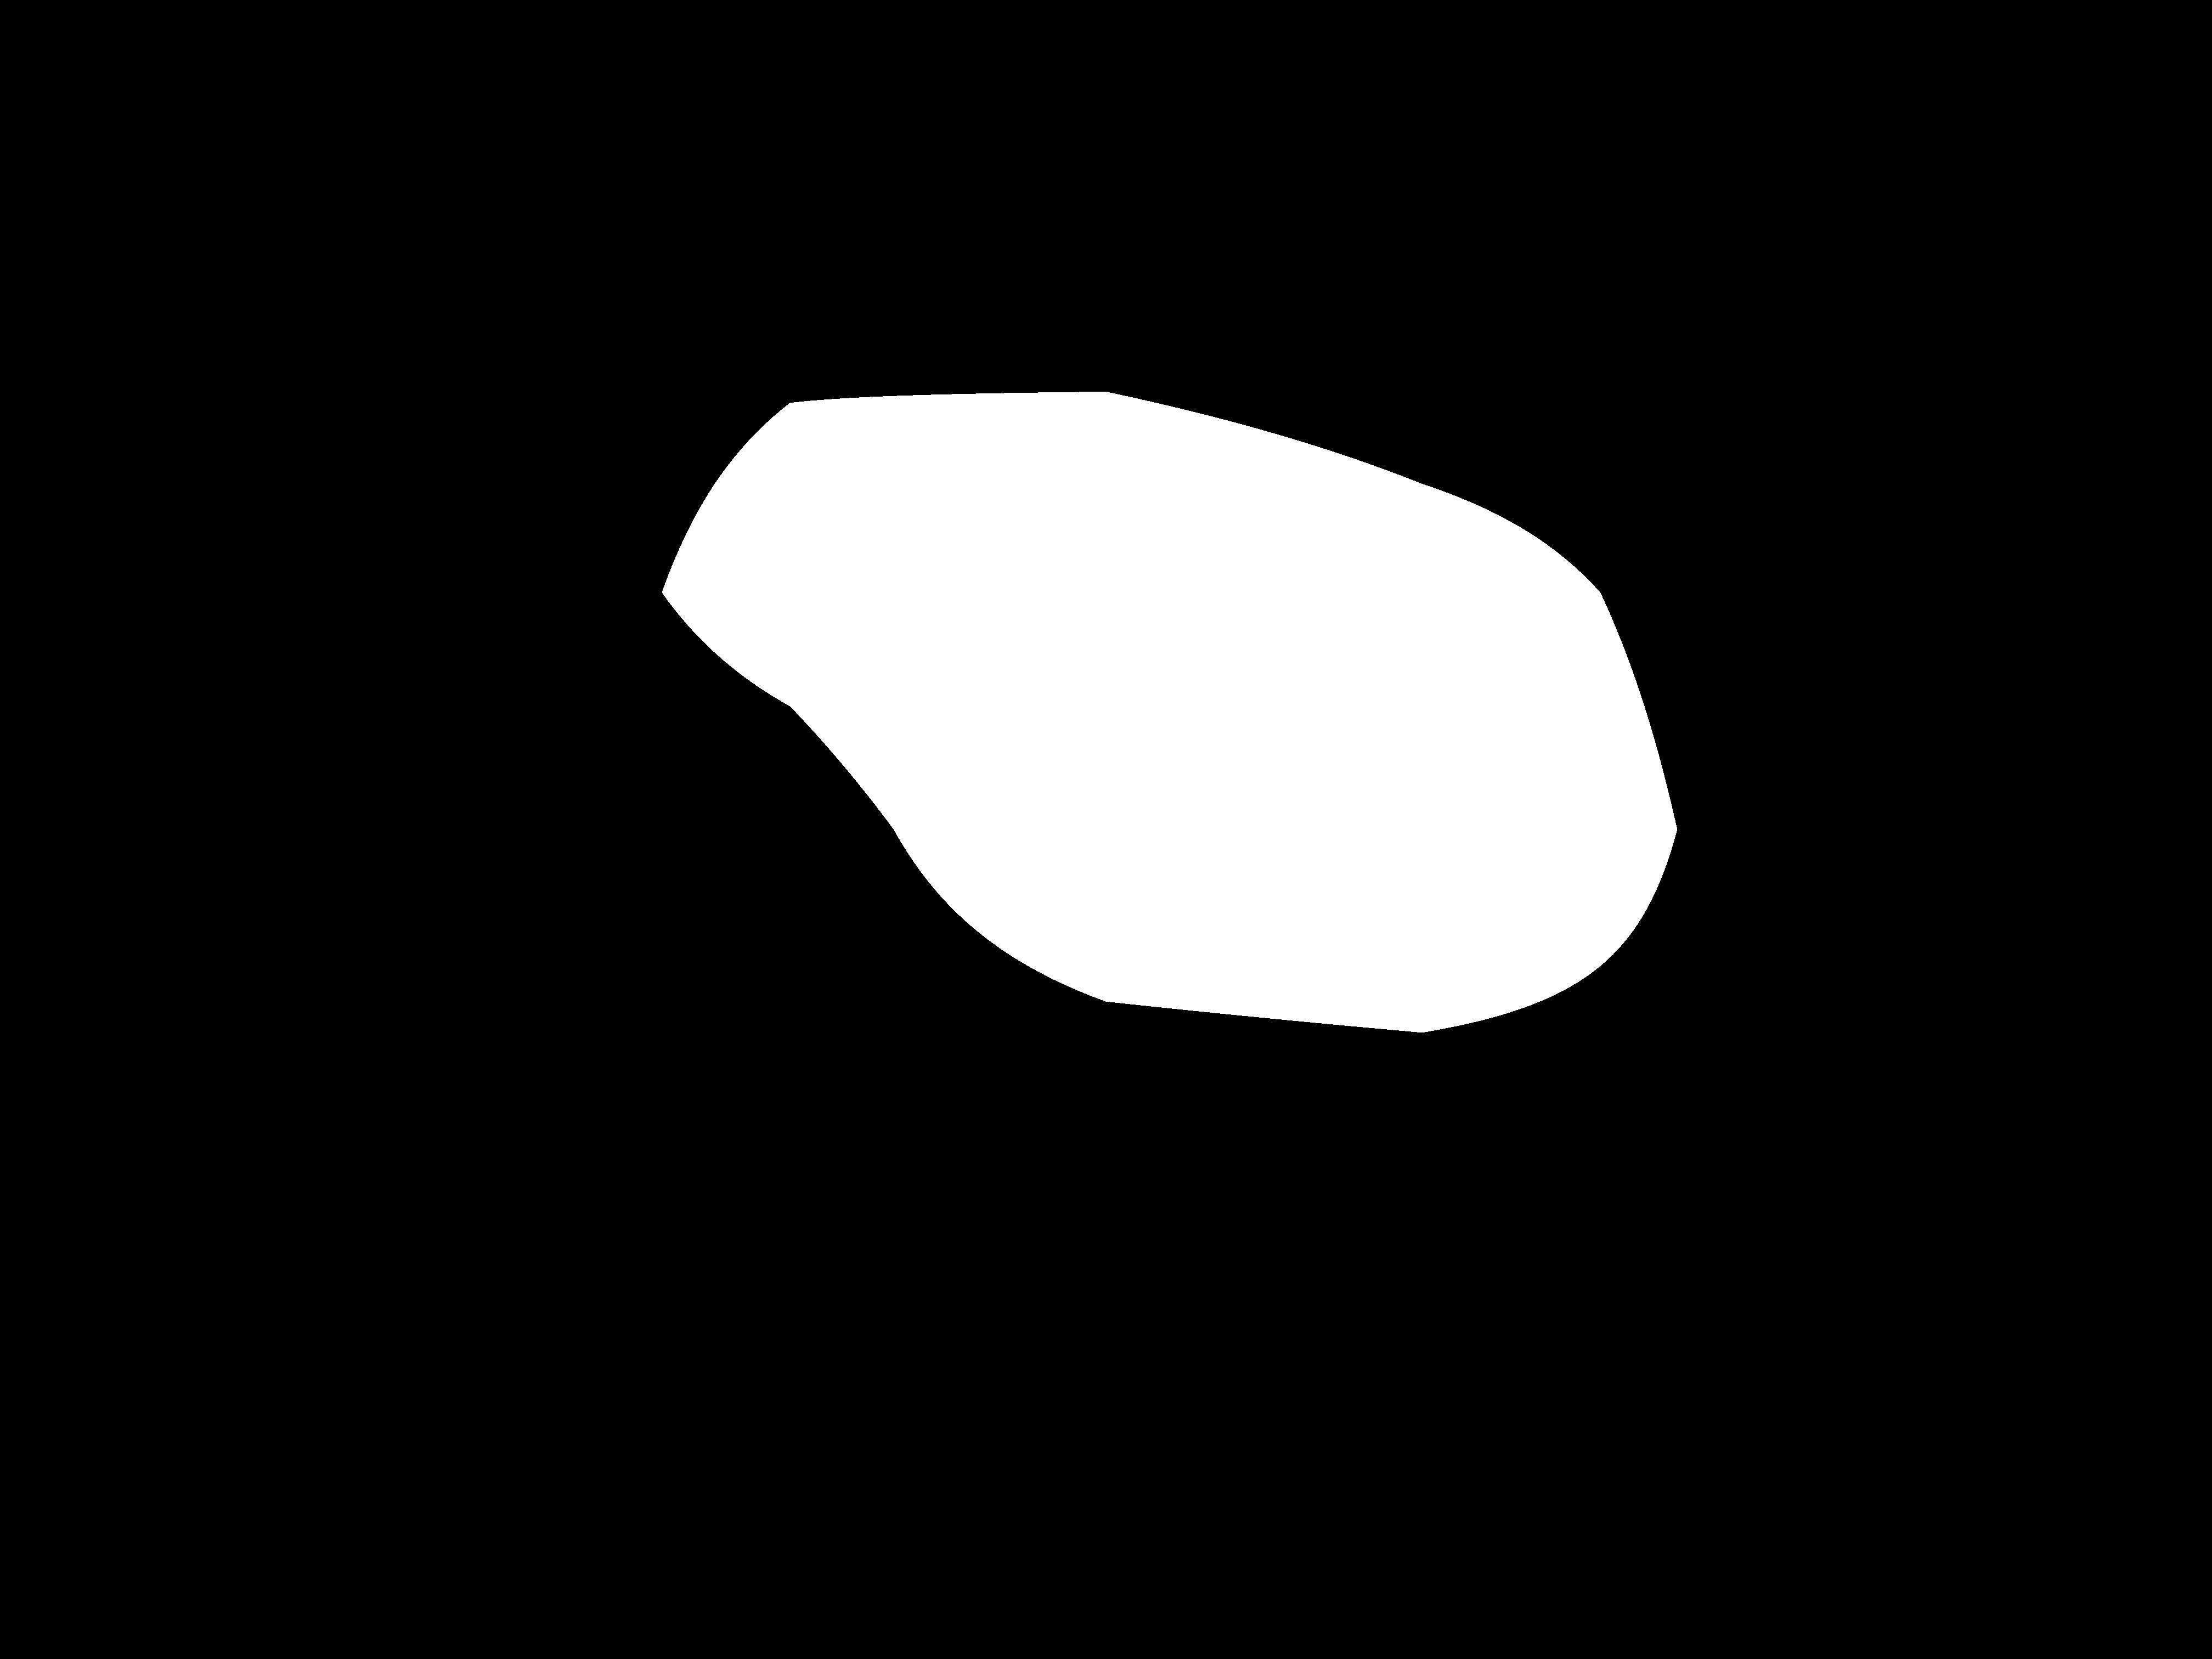
\includegraphics[height=2.5cm, width=2.5cm]{./attachments/results/0-calculator-seg.jpg}
          \caption{segmentation}
          \label{fig:heatmap resized}
      \end{subfigure}
      \caption{Results of \ac{grad-cam} on an image with multiple trained classes}
      \label{fig:grad cam mixed}
    \end{figure}
    Despite the vulnerability with localization, all four images were correctly classified.
\end{document}
